\documentclass[11pt]{article}
\usepackage{graphicx}
\usepackage[bookmarks=true]{hyperref}
\usepackage{bookmark}
\usepackage{hyperref}
\usepackage{float}
\usepackage{wrapfig}

\usepackage{array}
\newcolumntype{L}[1]{>{\raggedright\let\newline\\\arraybackslash\hspace{0pt}}m{#1}}
\newcolumntype{C}[1]{>{\centering\let\newline\\\arraybackslash\hspace{0pt}}m{#1}}
\newcolumntype{R}[1]{>{\raggedleft\let\newline\\\arraybackslash\hspace{0pt}}m{#1}}

\begin{document}

\begin{titlepage}
\begin{flushright}


\includegraphics[width=380px]{./images/University_of_Pretoria_Logo.png}
\newline
\newline

\textbf {\LARGE Software Requirements Specification} \newline

\textbf {\Large Linphone for Andriod Group Chat (Waterfall)}\newline

\textbf {\large Version: 2.0}\newline

\centering \textbf {\large Authors:}

\begin{table}[H]
\large
\centering
\begin{tabular}{rl}
	Izak Blom & 13126777 \\
	David Breetzke & 12056503 \\
	Paul Engelke & 13093500 \\
	Prenolan Govender & 13102380 \\
	Jessica Lessev & 13049136 \\
\end{tabular}
\end{table}

Date: 26 May 2015

\end{flushright}
\end{titlepage}

\setcounter{tocdepth}{3}
\tableofcontents

\newpage
\section{Revision History}
\begin{table}[h]
\begin{tabular}{llll}
\textbf{Date}          & \textbf{Description}  & \textbf{Author}       & \textbf{Comments}   \\ \hline
\multicolumn{1}{|R{2cm}|}{26/05/2015} & \multicolumn{1}{L{4.5cm}|}{Document Creation} & \multicolumn{1}{l|}{Team Eclectic} & \multicolumn{1}{L{4cm}|}{Version 1} \\ \hline
\multicolumn{1}{|l|}{} & \multicolumn{1}{l|}{} & \multicolumn{1}{l|}{} & \multicolumn{1}{l|}{} \\ \hline
\multicolumn{1}{|l|}{} & \multicolumn{1}{l|}{} & \multicolumn{1}{l|}{} & \multicolumn{1}{l|}{} \\ \hline
\multicolumn{1}{|l|}{} & \multicolumn{1}{l|}{} & \multicolumn{1}{l|}{} & \multicolumn{1}{l|}{} \\ \hline
\multicolumn{1}{|l|}{} & \multicolumn{1}{l|}{} & \multicolumn{1}{l|}{} & \multicolumn{1}{l|}{} \\ \hline
\multicolumn{1}{|l|}{} & \multicolumn{1}{l|}{} & \multicolumn{1}{l|}{} & \multicolumn{1}{l|}{} \\ \hline
\multicolumn{1}{|l|}{} & \multicolumn{1}{l|}{} & \multicolumn{1}{l|}{} & \multicolumn{1}{l|}{} \\ \hline
\multicolumn{1}{|l|}{} & \multicolumn{1}{l|}{} & \multicolumn{1}{l|}{} & \multicolumn{1}{l|}{} \\ \hline
\multicolumn{1}{|l|}{} & \multicolumn{1}{l|}{} & \multicolumn{1}{l|}{} & \multicolumn{1}{l|}{} \\ \hline
\multicolumn{1}{|l|}{} & \multicolumn{1}{l|}{} & \multicolumn{1}{l|}{} & \multicolumn{1}{l|}{} \\ \hline
\multicolumn{1}{|l|}{} & \multicolumn{1}{l|}{} & \multicolumn{1}{l|}{} & \multicolumn{1}{l|}{} \\ \hline
\multicolumn{1}{|l|}{} & \multicolumn{1}{l|}{} & \multicolumn{1}{l|}{} & \multicolumn{1}{l|}{} \\ \hline
\multicolumn{1}{|l|}{} & \multicolumn{1}{l|}{} & \multicolumn{1}{l|}{} & \multicolumn{1}{l|}{} \\ \hline
\multicolumn{1}{|l|}{} & \multicolumn{1}{l|}{} & \multicolumn{1}{l|}{} & \multicolumn{1}{l|}{} \\ \hline
\multicolumn{1}{|l|}{} & \multicolumn{1}{l|}{} & \multicolumn{1}{l|}{} & \multicolumn{1}{l|}{} \\ \hline
\end{tabular}
\end{table}

\section{Document Approval}
\begin{table}[h]
\begin{tabular}{llll}
\textbf{Signature}     & \textbf{Printed Name} & \textbf{Title}        & \textbf{Comments}     \\ \hline
\multicolumn{1}{|l|}{} & \multicolumn{1}{L{3.5cm}|}{} & \multicolumn{1}{L{3.5cm}|}{} & \multicolumn{1}{L{4cm}|}{} \\ \hline
\multicolumn{1}{|l|}{} & \multicolumn{1}{l|}{} & \multicolumn{1}{l|}{} & \multicolumn{1}{l|}{} \\ \hline
\multicolumn{1}{|l|}{} & \multicolumn{1}{l|}{} & \multicolumn{1}{l|}{} & \multicolumn{1}{l|}{} \\ \hline
\multicolumn{1}{|l|}{} & \multicolumn{1}{l|}{} & \multicolumn{1}{l|}{} & \multicolumn{1}{l|}{} \\ \hline
\end{tabular}
\end{table}

\newpage
\section{Introduction}

\subsection{Purpose}
The purpose of this document is to provide a detailed discussion of the Linphone Group Chat Extension system requirements and behaviour, in preparation for design and implementation. These requirements include use cases, functional and non-functional requirements as well as a description of the adjustments to be made to the existing user interfaces.
\subsection{Scope}
%The scope of this documentation is to cover all use cases and functional requirements that are necessary to provide group chat functionality to the Linphone service. \newline
%The scope of ManageGroups is restricted to creating, deleting and removing groups. These are further split up into lower-level use cases that are needed in order to achieve the desired functionality.
The scope of this document will cover the requirements of the features for the Linphone Group Chat Extension project, which are listed as follows:
\begin{itemize}
\item providing group chat capabilities such as:
\subitem  - creation and deletion of groups,
\subitem  - adding and removing members,
\subitem  - broadcasting all messages to all members,
\item sending messages using AES256 encryption for secure messaging,
\item sending messages without encryption where it is not needed,
\item sending voice recordings over IM,
\item making changes to the messaging user interface such as:
\subitem  - improving the spacing between words,
\subitem  - increasing the font sizes,
\subitem  - improving message indentation for sender clarity,
\subitem  - adding indication of another user typing a message,
\subitem  - improving user profile picture displays.
\end{itemize}
\begin{figure}[H]
\centering
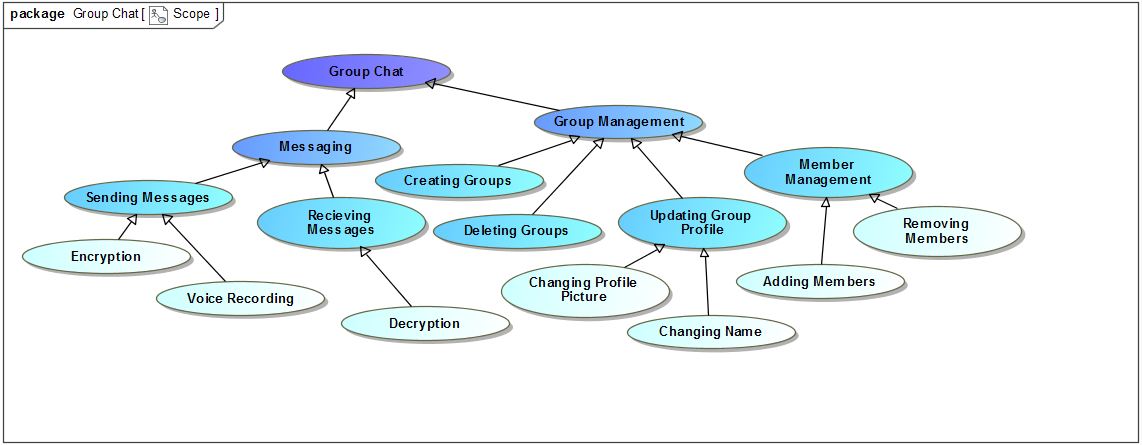
\includegraphics[width=5in]{./images/scope_master.png}
\caption[Group Chat Extension Scope]{This UML diagram shows the scope for the Linphone Group Chat extension.}
\label{figure-scope-master}
\end{figure}
\subsection{Definitions, Acronyms \& Abbreviations}
\subsubsection{Internal Documentation}
\paragraph{FR:} Stands for Functional Requirement. Functional requirements define the internal workings of the software to show how the use cases are satisfied.
\paragraph{NFR:} Stands for Non-functional Requirement. Non-functional requirements impose constraints on the design or implementation of the software.
\paragraph{UC:} Stands for Use Case. Use Cases describe the external behaviour of the software when a user interacts with it.
\subsubsection{External Documentation}
\paragraph{AES256:} AES stands for Advanced Encryption Standard and is a specification for encryption of electronic data. AES256 is a specific encryption algorithm that uses block sizes of 256 bits.
%\subsection{References}
\subsection{Overview}

\section{Specific Requirements}
%\subsection{External Interface Requirements}
\subsection{User Interfaces}
\paragraph{Group Chat Interface} The group chat interface will be implemented as an extension of the existing Linphone chat interface. This will involve the following modifications
\begin{itemize}
\item Displaying an indication that a subscribed user is busy typing
\item Improving word spacing on message displays
\item Increasing message font sizes
\item Improving message indentation for sender clarity
\item Associating a sender name to a message and displaying the name, since multiple users send messages via group chat.
\item Improving user profile picture displays
\end{itemize}
\paragraph{Group Chat Creation Interface} This interface will allow users to create a group for group chat purposes. Some parameters to be provided for editing on this interface:
\begin{itemize}
\item Enabling encryption
\item Group Name
\item Add a member functionality
\end{itemize}
\paragraph{Group Chat Settings Interface} This will be a specialisation of the Group Chat Creation Interface. Additionally functionality to remove a subscribed member from the group will be provided.

%\subsubsection{Hardware Interfaces}
%\subsubsection{Software Interfaces}
%\subsubsection{Communication Interfaces}
\newpage
\subsection{Use Cases}
\subsubsection{Create Group Chat} \label{UC-create-group}
\paragraph{Priority:}Critical
\paragraph{Summary:} A user creates a new group. This feature makes use of a number of other use cases to accomplish this goal.
\paragraph{Rationale:} The main aspect of the extension to the Linphone project is to provide group chat functionality. This feature gives the user the ability to create and initialize the group.
\paragraph{Users:}  Any Linphone user.
\paragraph{Preconditions:}For each of the pre-conditions below an exception is raised where that precondition is not met, to indicate service refusal.
The group will not be created if one of the following preconditions is not met:
\begin{itemize}
\item	User must have access to the Linphone service.
\item	The user may not create the group unless at least one other member is added.
\end{itemize}
\paragraph{{Postconditions:}}The post-conditions specify the conditions which must hold true when the service has been provided.
\begin{itemize}
\item	The creator is automatically assigned administrator rights.
\item	An invite is sent to the other added users to ask them if they want to be part of the group.
\item	The group is created with the respective profiles and members.
\end{itemize}
\begin{figure}[H]
\centering
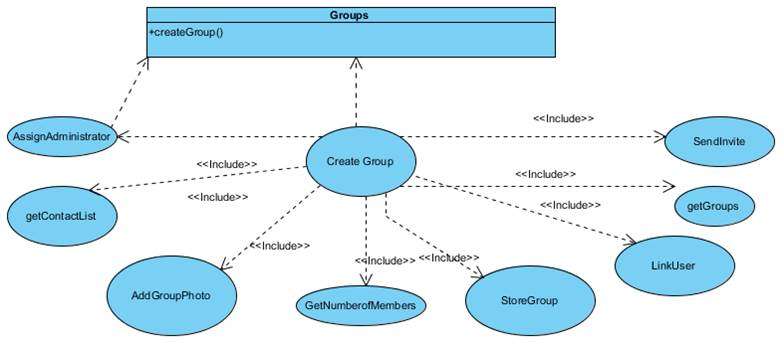
\includegraphics[width=5in]{./images/FR-create.jpg}
\caption[UC-figure-create-group]{A use case diagram for creating groups.}
\label{UC-figure-create-group}
\end{figure}
\textbf{Services Contract:}
\begin{itemize}
\item The CreateGroupRequest identifies the user that is creating the group and automatically assigns administrative rights to this user.
\item It allows the user to select contacts that the user wishes to add to the group.
\item The group members are then notified by receiving an invitation to join and are linked to the group, provided they accept the invite.
\item The service has three pre-conditions and three post-conditions.
\end{itemize}
\begin{figure}[H]
\centering
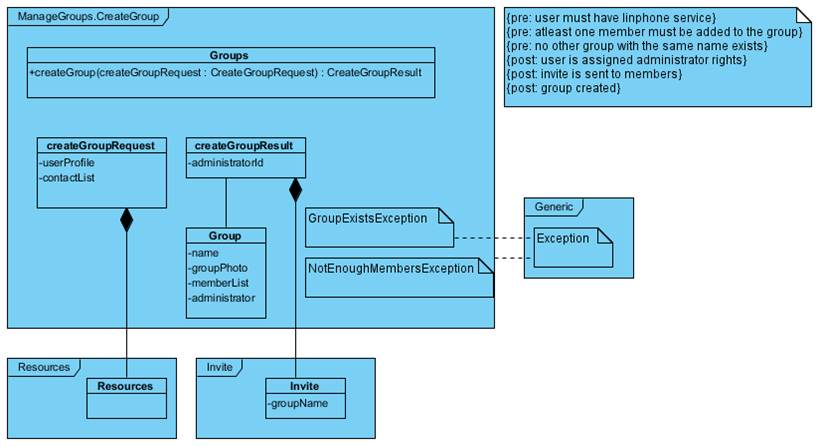
\includegraphics[width=5in]{./images/serviceContract-create.jpg} \newline
\caption[Create Group Services Contract]{A UML diagram showing the services contract for group creation.}
\label{SC-figure-create-group}
\end{figure}
%\paragraph{Included Use Cases} % this needs reformating, many of these should be functional requirements instead of use cases as the describe the inner workings of the create group use case.
% Use cases that are included are necessary to provide the lower level functionality needed in order to achieve the higher level functionality. These all deal with the resources and retrieving from storage. They  are:\newline
% \newline
% \textbf{addGroupPhoto  – Priority: Important} \newline
% \begin{itemize}
% \item	This use case allows a member of the group and the administrator, on group creation, to add a group photo. On group creation, if the creator does not specify a group photo, a default one is assigned.\newline
% \end{itemize}
% \textbf{getContactList – Priority: Important} \newline
% \begin{itemize}
% \item	This use case gets the user trying to create the group’s contact list and checks whether each contact added to the group has Linphone or not. If not an exception is thrown otherwise the system proceeds further.\newline
% \end{itemize}
% \textbf{getGroups  – Priority: Critical} \newline
% \begin{itemize}
%\item	This use case gets all the group names that the creator has in their chats list and checks that another group with the same name as the new group exists. If another group exists then an exception is thrown otherwise the system proceeds further. \newline
%\end{itemize}
 

\subsubsection{Send Invite} \label{UC-send-invite}
\paragraph{Summary:} Send Invite is triggered when a group is created with new members or when a new member is added to the group. The invite informs the user that they are added to a group and can either accept it or decline it.
\paragraph{Rationale:} It is done so that new members can join a group chat.
\paragraph{Preconditions:}
 For each of the pre-conditions below an exception is introduced which is raised by the service to notify the caller that the service is not being provided as the pre-condition associated with that exception has not been met.\newline
 The invite will not be sent if one of the following scenarios occurs:
 \begin{itemize}
 \item	The receiver of the invite is not a contact added by the administrator of the group.
 \end{itemize}
\paragraph{Postconditions:}
The post-conditions specify the conditions which must hold true when the service has been provided.
 \begin{itemize}
\item	The invite must be sent to the correct user.
\end{itemize}
\begin{figure}[H]
\centering
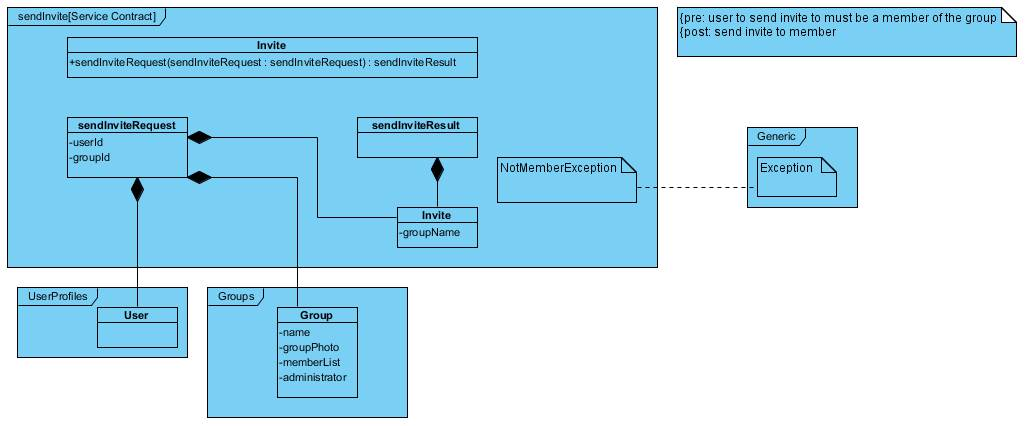
\includegraphics[width=5in]{./images/serviceContract-sendInvite.jpg}
\caption[Send Invite Services Contract]{A UML services contract for the Send Invite use case.}
\label{SC-figure-send-invite}
\end{figure}
\begin{figure}[H]
\centering
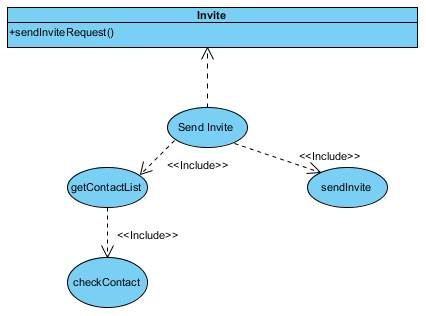
\includegraphics[width=3in]{./images/FR-sendInvite.jpg}
\caption[Send Invite Use Case Diagram]{A UML use case diagram for Send Invite.}
\end{figure}

\subsubsection{Delete Group Chat} \label{UC-delete-group}
\paragraph{Priority:}Critical
\paragraph{Summary:}A user can leave a group chat. When all the users leave a group chat, it will be deleted. If only one person remains in a group chat, that person will be unable to send messages to the chat until at least one other person is added to the chat. If the group owner leaves the group, a new owner is automatically assigned.
\paragraph{Rationale:}When an owner of a group leaves the group, the administrative privileges need to be reallocated. The group chat should persist as long as there is at least one user in the group. In the case of only one user remaining, preventing that user from sending messages will guard against misuse of the group chat, as well acting as an alert that the user's message would not have been seen by any other users.
\paragraph{Users:} Any user of the Linphone application.
\paragraph{Preconditions:} The user must be part of a group.
\paragraph{{Postconditions:}} 
\begin{itemize}
	\item User leaving is the administrator:
\end{itemize}
%\includegraphics[]{name} -- for use case diagram

\subsubsection{Update Group Chat Profile} \label{UC-update-group}
\paragraph{Priority:} Important
\paragraph{Summary:}
The group name, subject, and profile picture can be changed.
\paragraph{Rationale:}
The nature of groups can change when members are added or removed, resulting in name and subject changes. Users tend to update profile pictures often in order to keep groups from growing stale or to have the picture relate to the group name or subject. Allowing users to update features of the group will allow groups to be easier to manage and usable in terms of aesthetics.
\paragraph{Users:}
Any member of the group.
\paragraph{Preconditions:}
A group exists and has members.
\paragraph{{Postconditions:}}
The current name, subject, or profile picture has been changed.
%\includegraphics[]{name} -- for use case diagram

\subsubsection{Add Member} \label{UC-add-member}
\paragraph{Priority:} Critical
\paragraph{Summary:}
A user is added to the list of users currently in the group.
\paragraph{Rationale:}
The group does not have a static amount of users, this is inefficient. If the creator of the group has forgotten to add a user to the group after initial creation, the creator should still be able to add the user later. Should a user relevant to the group appear after creation of the group, the user should still be able to join the group. In addition, should a user leave, the user should be able to come back to the group.
\paragraph{Users:}
Creator or the current administrator of the group.
\paragraph{Preconditions:}
Group exists with an administrator in it.
\paragraph{{Postconditions:}}
The user is added to the list of current users in the group and receives messages, etc.
%\includegraphics[]{name} -- for use case diagram

\subsubsection{Remove Member} \label{UC-remove-member}
\paragraph{Priority:} Critical
\paragraph{Summary:}
A user is removed from the list of users currently in the group.
\paragraph{Rationale:}
Should a user be added to the group accidentally, it should be possible to remove said user. Users should additionally be able to remove themselves from the group should they no longer require it. Being able to remove users and users being able to remove themselves aides in the management of the group.
\paragraph{Users:}
All users. (Administration can remove other users, all users can remove themselves.)
\paragraph{Preconditions:}
A group exists with more than one member.
\paragraph{{Postconditions:}}
The user is no longer a part of the group which entails the user not receiving messages from the group, etc.
\begin{figure}[H]
\centering
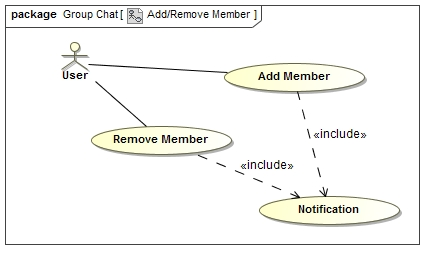
\includegraphics[width=5in]{./images/UC_AddRemove_Member.jpg}
\caption[Add/Remove Member use case]{This UML case diagram shows the use case for adding and removing members combined as both are simple and utilise essentially the same use case.}
\label{UC-figure-addremove-member}
\end{figure}

\subsubsection{Change Administrator} \label{UC-change-admin}
\paragraph{Priority:} Important
\paragraph{Summary:}
Removes administrator privileges from the current administrator and reassigns to another user within the group.
\paragraph{Rationale:}
If a user prefers not to be administrator anymore or the current administrator would like to leave the group, assigning a new user within the group with administrator privileges makes management of the group easier.
\paragraph{Users:}
Administrator of the group.
\paragraph{Preconditions:}
Group exists with an administrator and at least one other user.
\paragraph{{Postconditions:}}
The user selected receives administrator privileges while the current administrator is stripped of the privileges.
%\includegraphics[]{name} -- for use case diagram

\subsubsection{Send Message} \label{UC-send-message}
\paragraph{Priority:} Critical
\paragraph{Summary:} The message object shall be broadcast to all participants of the group chat.
\paragraph{Rationale:} The purpose of a group chat is to provide a central point of communication for a group of people. A user should thus be able to convey a message to all other participant users in one single action.
\paragraph{Users:} Any registered member of the group chat.
\paragraph{Preconditions:} 
\begin{itemize}
\item The user is a member of the group chat.
\item The interface that has focus, is the group chat interface.
\end{itemize}
\paragraph{{Postconditions:}}
\begin{itemize}
\item The user's message has been sent to all other participants.
\end{itemize}

\subsubsection{Receive Message} \label{UC-receive-message}
\paragraph{Priority:} Critical
\paragraph{Summary:} A message object sent on a group is received by every member subscribed to a group.
\paragraph{Rationale:} After a message has been broadcast to all members subscribed/linked to a group, each member should be able to receive the message upon receiving a broadcast request. This involves analysing and displaying the message using the appropriate interface. 
\paragraph{Users:} Any registered member of the particular group on which a message is broadcast.
\paragraph{Preconditions:} 
\begin{itemize}
\item A message object has been broadcast to all users subscribed to a particular group.
\item The user receiving an incoming message should be subscribed to the group from which the message is broadcast.
\end{itemize}
\paragraph{{Postconditions:}}
\begin{itemize}
\item The message is analysed/parsed
\item The message is displayed on the group chat interface
\end{itemize}
\begin{figure}[H]
\centering
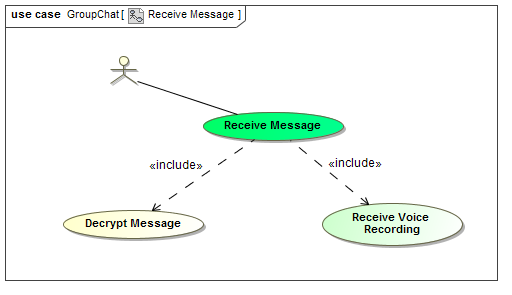
\includegraphics[width=5in]{./images/UC_Receive_Message.png}
\caption[Receive Message Use Case Diagram]{This use case diagram shows receive message and receive voice recording together.}
\label{FR-figure-create-group}
\end{figure}
\paragraph{References:} UC \ref{UC-receive-voice}

\subsubsection{Send Voice Recording} \label{UC-send-voice}
\paragraph{Priority:} Important
\paragraph{Summary:} A user will be able to record voice messages and send them via IM.
\paragraph{Rationale:} A user may be pressed for time, unable type a message, or the recipient may be unable to read the message, due to some external factor and thus require a means other than text messaging to convey a message. The ability to record one's voice and send the recording as a message may cater for the described scenarios and more.
\paragraph{Users:} Any user of the Linphone application.
\paragraph{Preconditions:} The user's device must support voice recording --- the device requires a microphone to support this.
\paragraph{{Postconditions:}} A message has been sent to the recipient containing the voice recording.
\begin{figure}[H]
\centering
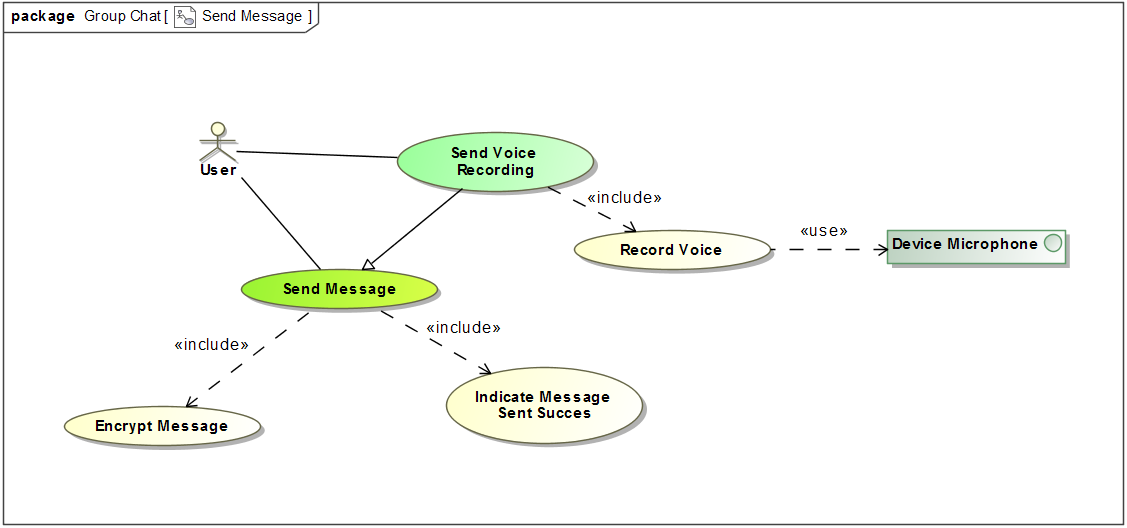
\includegraphics[width=5in]{./images/send_message_UC.png}
\caption[Send Message Use Case]{This UML case diagram shows the use case for Send Message and Send Voice Recording in combination as Send Voice Recording is essentially an specialization of Send Message.}
\label{UC-figure-send-message}
\end{figure}

\subsubsection{Receive Voice Recording} \label{UC-receive-voice}
\paragraph{Priority:} Important
\paragraph{Summary:} A user will be able to record voice messages and send them via IM. Other users should be able to receive this message type and listen to it.
\paragraph{Rationale:} Voice messages sent over group chat should be receivable by all members linked to the group. Members should be able to download and listen to the message.
\paragraph{Users:} Any user of the Linphone application having received a voice message.
\paragraph{Preconditions:} 
\begin{itemize}
\item The user's device must be connected to the internet and Linphone server.
\item The user's device must be able to play the received voice recording.
\end{itemize}
\paragraph{{Postconditions:}} The voice recording has been downloaded and is available for playback.
%\includegraphics[]{name} -- for use case diagram

\newpage

\subsection{Functional Requirements}
\subsubsection{Create Group Chat} \label{FR-create-group}
\paragraph{Summary:} The create group use case should allow a user who has the Linphone service to create a group, name it, set details such as the profile picture and add contacts to it.
\paragraph{Rationale:} A user may need a central way of communicating with several users at a time and wish to have a way of communicating and exchanging messages with several people at a time and observe their replies to each other etc. Thus a group chat is needed.
\paragraph{Requirements:} When the user decides to create a group, the user must be afforded the option to do so. Once selected the user must be provided with the opportunity to give the group a name and picture. The system should check the validity of the above activities and then allow the user to proceed if all options are valid. The user should then be allowed to add contacts to the group. Once more than one contact is added the user is allowed to continue and finish creating the group.
\begin{figure}[H]
\centering
\includegraphics[width=5in]{./images/process-create.jpg}
\caption[Create Group Activity Diagram]{An activity diagram showing the group creation process.}
\label{FR-figure-create-group}
\end{figure}
\paragraph{References:} UC \ref{UC-delete-group}

\subsubsection{Send Invite} \label{FR-invite}
\paragraph{Summary:}
\paragraph{Rationale:}
\paragraph{Requirements:}
\paragraph{References:} UC \ref{}
 \begin{figure}[H]
 \centering
 \includegraphics[width=3in]{./images/process-sendInvite.jpg}
 \caption[Send Invite Activity Diagram]{An activity diagram for the Send Invite use case.}
 \label{FR-figure-send-invite}
 \end{figure}
 
\subsubsection{Delete Group Chat} \label{FR-delete-group}
\paragraph{Summary:}
\paragraph{Rationale:}
\paragraph{Requirements:}
\paragraph{References:} UC \ref{UC-delete-group}

\subsubsection{Update Group Profile Picture} \label{FR-update-group-picture}
\paragraph{Summary:}
Updating should allow a user to remove the profile picture from the group or choose an image from local storage to replace the current profile picture.
\paragraph{Rationale:}
A user will often change the profile picture of the group, allowing the user to choose an image from local storage will afford the user more options.
\paragraph{Requirements:}
When the user chooses to change the profile picture, the user must be afforded the option to remove the profile picture (replacing it with a default system image) or allow the user to choose a new picture by invoking the file manager in order to choose a picture from local storage. The updated profile picture should be visible to all users within the group after the change has taken place.
\paragraph{References:} UC \ref{UC-update-group}

\subsubsection{Add Member} \label{FR-add-member}
\paragraph{Summary:}
Once the user has been added to the group, the user must be able to receive messages from the group and other members.
\paragraph{Rationale:}
Users will be added at different times to other users therefore it must be guaranteed that each user receives the same messages as other group members.
\paragraph{Requirements:}
Once the administrator opts to add a user, the list of contacts the user currently has must appear and the user can choose another user to add to the group. When the user is selected, that user must be added to the group list and receive all messages sent in the group from that point.
\paragraph{References:} UC \ref{UC-add-member}

\subsubsection{Remove Member} \label{FR-remove-member}
\paragraph{Summary:}
Once the user has been removed from the group, the user must not receive any messages from the group.
\paragraph{Rationale:}
Users will be removed at different times to other users therefore it must be guaranteed that the user who is removed does not receive any messages from the group to ensure that the user is not a part of the group.
\paragraph{Requirements:}
Once the administrator opts to remove a user from the list of users currently in the group, the user selected must be removed from the group and should no longer receive any messages from the group.
\paragraph{References:} UC \ref{UC-remove-member}

\subsubsection{Encryption for Send Message} \label{FR-send-message-encrypted}
\paragraph{Summary:} The send message feature shall provide for encryption.
\paragraph{Rationale:} If the group administrator decides that messages should be encrypted for secure communication amongst members, the ability to do so shall be provided.
\paragraph{Requirements:} When encryption is enabled, the send message feature shall use the AES265 encryption algorithm to encrypt the message before broadcasting it to the group members. If encryption is not enabled, the message will be broadcast in it's original state.
\paragraph{References:} UC \ref{UC-send-message}

\subsubsection{Sent Message Indication} \label{FR-send-message-indicator}
\paragraph{Summary:} The send message feature shall provide indication of a successful broadcast or the failure thereof.
\paragraph{Rationale:} Users need to know whether or not their messages have been sent else they must assume one or the other, and that is not reliable. If some indication is given of the success of sending a message, a user will be able to take any necessary action in the event of a failure.
\paragraph{Requirements:} When a user invokes the send message feature, the feature will provide an indication of the success after completing it's execution.
\paragraph{References:} UC \ref{UC-send-message}

\subsubsection{Voice Recording Support} \label{FR-voice-record-support}
\paragraph{Summary:} The voice recording feature shall check that the device has a microphone.
\paragraph{Rationale:} The voice recording feature can only operate if it can receive audio input from the device's microphone. Without such a check, trying to access the feature can lead to the possibility of a system crash.
\paragraph{Requirements:} When the voice recording feature is invoked, the procedure will check that the device can record audio. If it can, it will proceed with normal execution: using the device microphone to record the audio and once done, wrap the audio file in a message object and send it; else it will abort the process and alert the user that the feature is not available.
\paragraph{References:} UC \ref{UC-send-voice}

\subsubsection{Decryption of Received Message} \label{FR-decrypt-received-message}
\paragraph{Summary:} Decryption of received messages is required before display and further processing.
\paragraph{Rationale:} Group administrators can enable encryption for all messages sent on the group. These messages are encrypted before being sent and should be decrypted after received.
\paragraph{Requirements:} When encryption is enabled, the send message feature shall use the AES265 encryption algorithm to encrypt the message before broadcasting it to the group members. In this case, the AES265 algorithm will also be used to decrypt the message once received by members subscribed to the group, given that encryption for messages sent on the group is enabled.
\begin{figure}[H]
\centering
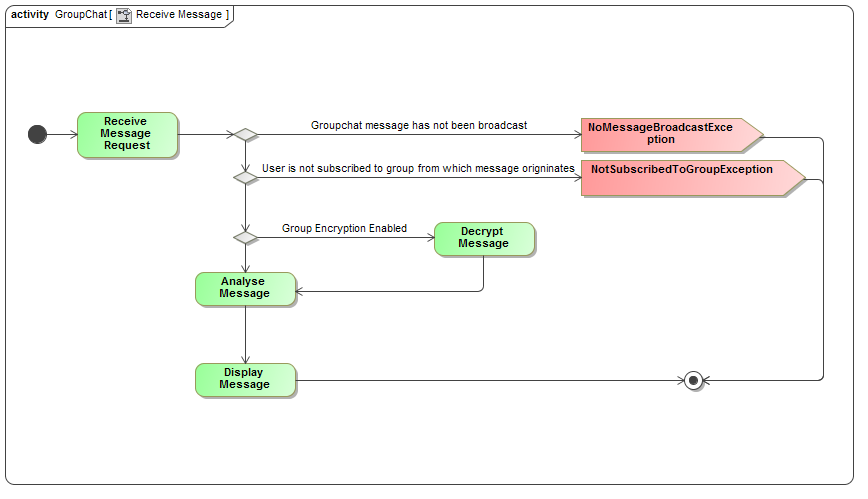
\includegraphics[width=5in]{./images/Activity_Receive_Message.png}
\caption[Receive Message Activity Diagram]{An activity diagram showing the receive message process and the  usage of encryption in process flow.}
\label{FR-figure-activity-receive-message}
\end{figure}
\paragraph{References:} UC \ref{UC-delete-group}

\newpage
\subsection{Non-Functional Requirements}

\subsubsection{Scalability Constraints for Add User} \label{NFR-scalability-add-member}
\paragraph{Summary:} Adding a new user may not negatively impact the performance of management of, and communication within, the group.
\paragraph{Rationale:} If there are too many members in a group, it can become hard for the group administrator to keep track of members and there may be noticeable delays in message broadcasting with some users receiving messages much later than others. This can impact the service quality negatively cause people to stop using the service.
\paragraph{Requirements:} The number of users per group shall be limited to a reasonable size to prevent poor performance. This number should be between 50 and 100 users, although this number is subject to change as development and testing progress.
\paragraph{References:} UC \ref{UC-add-member}

\subsubsection{Performance Constraints for Send Message} \label{NFR-performance-send-message}
\paragraph{Summary:} Sending messages should be quick.
\paragraph{Rationale:} Broadcasting messages to the entire group should be quick for effective communication to take place. If broadcasting a message to the group is slow, the quality of the real-time communication experience becomes poor and may cause users to avoid the use of the service. 
\paragraph{Requirements:} Messages should be sent to all group members within reasonable time, but as fast as possible. The time within which the message should be received should be about 5 seconds. However, factors to take into account may include user availability (the user may be off-line) and network congestion and/or connection issues. Refer to NFR \ref{NFR-reliability-send-message} for details on reliability of Send Message.
\paragraph{References:} UC \ref{UC-send-message}

\subsubsection{Reliability Constraints for Send Message} \label{NFR-reliability-send-message}
\paragraph{Summary:} The send message feature should be reliable, indicating failed or successful message broadcasts.
\paragraph{Rationale:} Users should be notified if their message was sent or not, allowing them to take the necessary action to complete their communication. If a user does not receive some form of confirmation of success or failure, the user will have to assume that the message was sent even if or when it was not, resulting in an unreliable service.
\paragraph{Requirements:} The send message feature shall provide some indication of success after perform its tasks.
\paragraph{References:} UC \ref{UC-send-message}, FR \ref{FR-send-message-indicator}

\subsubsection{Security Constraints for Send Message and Receive Message} \label{NFR-security-send-message-and-receive-message}
\paragraph{Summary:} The sending and receiving of message should be secured through reliable encryption and decryption.
\paragraph{Rationale:} Messages are required to be encrypted if the group administrator indicates this requirement during group creation. Encryption of sent messages and subsequent decryption of all received messages is required using the AES 256 encryption algorithm. 
\paragraph{Requirements:} The send message use case will incorporate encryption as a functional requirement and the receive message use case will incorporate decryption as a functional requirement.
\paragraph{References:} UC \ref{UC-send-message}, UC \ref{UC-receive-message}, FR \ref{FR-send-message-encrypted}, FR \ref{FR-decrypt-received-message}

\subsubsection{Availability Constraints for Receive Message} \label{NFR-availability-receive-message}
\paragraph{Summary:} A Linphone client should be able to receive a message whenever a message has been sent to it.
\paragraph{Rationale:} Although already implemented, the receive message use case needs to incorporate decryption of a received message using the AES256 protocol and will therefore be modified or integrated with a decryption implementation. Evoking a receive request should maintain high availability, since many messages can be sent in sequence during a group chat session.
\paragraph{Requirements:} Evoking a receive request should maintain high availability in the form of multi-threading or a similar technique.
\paragraph{References:} UC \ref{UC-receive-message}, FR \ref{FR-decrypt-received-message}


%\section{Requirements Traceability Matrix}

\newpage
\section{Appendix A} \label{appendix-a}
\listoffigures

\end{document}